% These are examples of how to work flow charts in the tikz package


\documentclass[10pt,titlepage]{article}
\usepackage{amsmath,amsthm,amsfonts,amssymb,amsbsy,graphicx,enumerate,marvosym}
\usepackage{tikz}\usetikzlibrary{shapes,arrows,positioning,calc,fit}
\usepackage{fullpage}
\usepackage{geometry}
\usepackage{pdflscape}

\pagestyle{empty}

\newgeometry{margin=1cm}

%-- Flow Chart Definitions -----------------------------------------
\tikzstyle{cloud} = [rectangle, draw, fill=red!20, inner sep=0.25em, text width=5em, text centered, rounded corners, minimum height=4em, execute at begin node=\scriptsize]
\tikzstyle{subcloud} = [rectangle, draw, fill=green!20, inner sep=0.5em, text width=8em, text centered, rounded corners, minimum height=3em, execute at begin node=\scriptsize]
\tikzstyle{block} = [rectangle, draw, fill=blue!20, inner sep=0.5em, text width=13em, align=center, minimum height=3em, execute at begin node=\scriptsize]
\tikzstyle{light} = [rectangle, draw, fill=blue!10, inner sep=0.5em, text width=9em, text centered, minimum height=1em, execute at begin node=\tiny]
\tikzstyle{io} = [trapezium, draw, fill=green!20, trapezium left angle=70, trapezium right angle=-70, inner sep=0.5em, text width=5em, text centered, minimum height=3em, execute at begin node=\scriptsize]
\tikzstyle{decision} = [diamond, draw, fill=yellow!20, inner sep=0.05em, aspect=2, text width=4em, text badly centered, minimum height=5em, minimum width=7em, rounded corners, execute at begin node=\tiny]
\tikzstyle{query} = [rectangle, draw, fill=red!20, inner sep=0.5em, text width=5em, text centered, minimum height=3em, execute at begin node=\scriptsize]
\tikzstyle{prompt} = [trapezium, draw, fill=green!20, trapezium left angle=60, trapezium right angle=60, inner sep=0.5em, text width=5em, text centered, minimum height=3em, execute at begin node=\scriptsize]
\tikzstyle{stop} = [regular polygon, regular polygon sides=8, draw, fill=red!20, inner sep=0.05em, text width=5em, text centered, execute at begin node=\scriptsize]
\tikzstyle{go} = [circle, draw, fill=green!20, inner sep=0.5em, text width=5em, text centered, rounded corners, minimum height=3em, execute at begin node=\scriptsize]


\tikzstyle{line} = [draw, -latex']
\tikzstyle{noarrow} = [draw]
\tikzstyle{container} = [rectangle, draw, inner sep=0.4em, dashed, fill=none, color=red!40]
%-------------------------------------------------------------------

\begin{document}

% begin flow diagram for ODE
\begin{figure} [htbp] \centering
	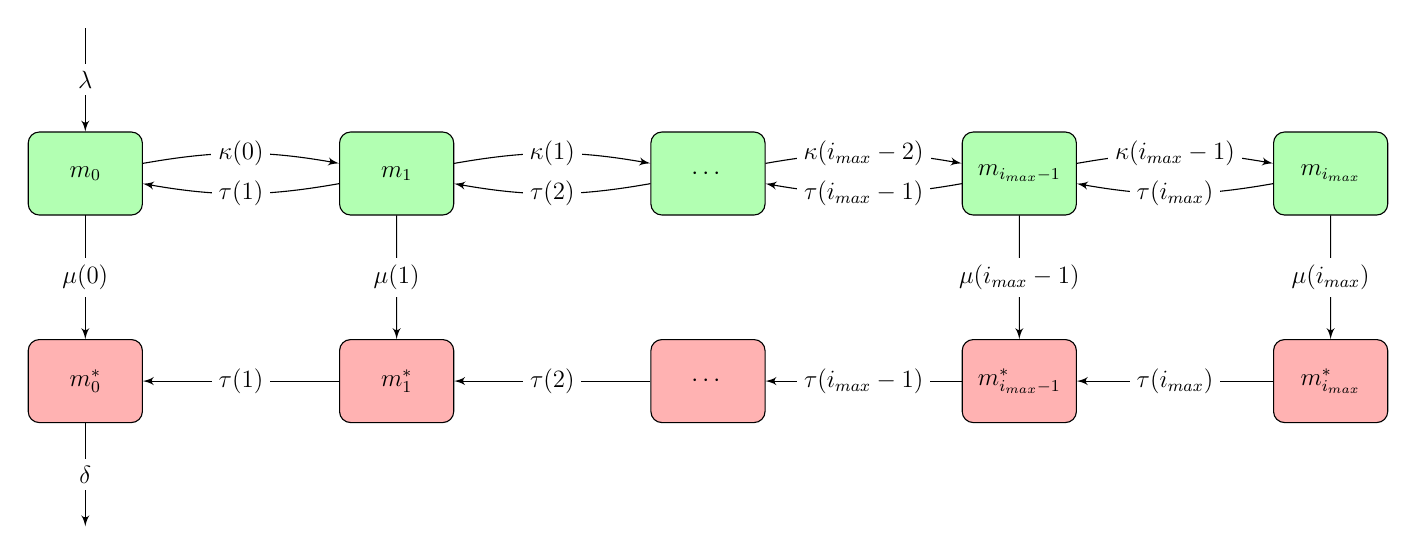
\begin{tikzpicture}[every node/.style={rectangle,fill=white,node distance=16ex, scale=0.75}, scale=0.90]
		% Row 1
		\node[cloud, fill=green!30](m0) {\large $m_0$};
		\node[cloud, fill=green!30, right of = m0, node distance = 15em](m1){\large $m_1$};
		\node[cloud, fill=green!30, right of = m1, node distance = 15em](cdots1){\large $\cdots$};
		\node[cloud, fill=green!30, right of = cdots1, node distance = 15em](mimaxn){\large $m_{i_{max}-1}$};
		\node[cloud, fill=green!30, right of = mimaxn, node distance = 15em](mimax){\large $m_{i_{max}}$};
		
		% Row 2
		\node[cloud, fill=red!30, below of = m0, node distance = 10em](m*0) {\large $m^*_0$};
		\node[cloud, fill=red!30, below of = m1, node distance = 10em](m*1){\large $m^*_1$};
		\node[cloud, fill=red!30, below of = cdots1, node distance = 10em](cdots2){\large $\cdots$};
		\node[cloud, fill=red!30, below of = mimaxn, node distance = 10em](m*imaxn){\large $m^*_{i_{max}-1}$};
		\node[cloud, fill=red!30, below of = mimax, node distance = 10em](m*imax){\large $m^*_{i_{max}}$};
		
		% empty nodes for input and output flow arrows		
		\coordinate[above of=m0, node distance=7em] (lambda);
		\coordinate[below of=m*0, node distance=7em] (delta);
		
		% Paths
		\path [line] (lambda) -- node[]{\large $\lambda$} (m0);
		\path [line] (m0) to [bend left=10] node{\large $\kappa(0)$} (m1);
		\path [line] (m1) to [bend left=10] node{\large $\kappa(1)$} (cdots1);
		\path [line] (cdots1) to [bend left=10] node{\large $\kappa(i_{max}-2)$} (mimaxn);
		\path [line] (mimaxn) to [bend left=10] node{\large $\kappa(i_{max}-1)$} (mimax);
		\path [line] (m1) to [bend left=10] node{\large $\tau(1)$} (m0);
		\path [line] (cdots1) to [bend left=10] node{\large $\tau(2)$} (m1);
		\path [line] (mimaxn) to [bend left=10] node{\large $\tau(i_{max}-1)$} (cdots1);
		\path [line] (mimax) to [bend left=10] node{\large $\tau(i_{max})$} (mimaxn);
		\path [line] (m0) -- node[]{\large $\mu(0)$} (m*0);
		\path [line] (m1) -- node[]{\large $\mu(1)$} (m*1);
		%Options for middle path between (...)
		%\path [line] (cdots1) -- (cdots2);
		%\path [line] (cdots1) -- node[]{\large $\mu(\cdots)$} (cdots2);
		\path [line] (mimaxn) -- node[]{\large $\mu(i_{max}-1)$} (m*imaxn);
		\path [line] (mimax) -- node[]{\large $\mu(i_{max})$} (m*imax);
		\path [line] (m*1) -- node[]{\large $\tau(1)$} (m*0);
		\path [line] (cdots2) -- node[]{\large $\tau(2)$} (m*1);
		\path [line] (m*imaxn) -- node[]{\large $\tau(i_{max}-1)$} (cdots2);
		\path [line] (m*imax) -- node[]{\large $\tau(i_{max})$} (m*imaxn);
		\path [line] (m*0) -- node[]{\large $\delta$} (delta);
		
	\end{tikzpicture}
\end{figure}
\pagebreak



% The most simple diagram
\begin{figure} [htbp] \centering
	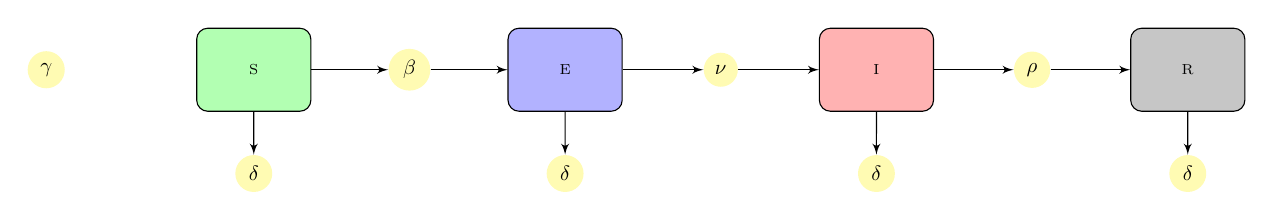
\begin{tikzpicture}[every node/.style={rectangle,fill=white,node distance=16ex, scale=0.75}, scale=0.90]
		% Row 1
		\node[circle, fill=yellow!30] (Births){$\gamma$};
		\node[cloud, fill=green!30, right of = Births, node distance = 10em](Susceptible) {S};
		\node[circle, fill=yellow!30, right of = Susceptible, node distance = 7.5em] (EffectiveTransmission){$\beta$};
		\node[cloud, fill=blue!30, right of = Susceptible, node distance = 15em](Exposed){E};
		\node[circle, fill=yellow!30, right of = Exposed, node distance = 7.5em] (Infectious){$\nu$};
		\node[cloud, fill=red!30, right of = Exposed, node distance = 15em](Infected){I};
		\node[circle, fill=yellow!30, right of = Infected, node distance = 7.5em] (Cure){$\rho$};
		\node[cloud, fill=darkgray!30, right of = Infected, node distance = 15em](Removed){R};
		
		% Row 2
		\node [circle, fill=yellow!30, below of = Susceptible, node distance = 5em](delta1){$\delta$};
		\node [circle, fill=yellow!30, below of = Exposed, node distance = 5em](delta2){$\delta$};
		\node [circle, fill=yellow!30, below of = Infected, node distance = 5em](delta3){$\delta$};
		\node [circle, fill=yellow!30, below of = Removed, node distance = 5em](delta4){$\delta$};
		
		% Paths
		\path [line] (Births)  (Susceptible);
		\path [line] (Susceptible) -- (EffectiveTransmission);
		\path [line] (EffectiveTransmission) -- (Exposed);
		\path [line] (Exposed) -- (Infectious);
		\path [line] (Infectious) -- (Infected);
		\path [line] (Infected) -- (Cure);
		\path [line] (Cure) -- (Removed);
		\path [line] (Susceptible.south) -- (delta1.north);
		\path [line] (Exposed.south) -- (delta2.north);
		\path [line] (Infected.south) -- (delta3.north);	
		\path [line] (Removed.south) -- (delta4.north);
		
	\end{tikzpicture}
\end{figure}
\pagebreak

% A little complex
\begin{figure}[htbp] \centering
	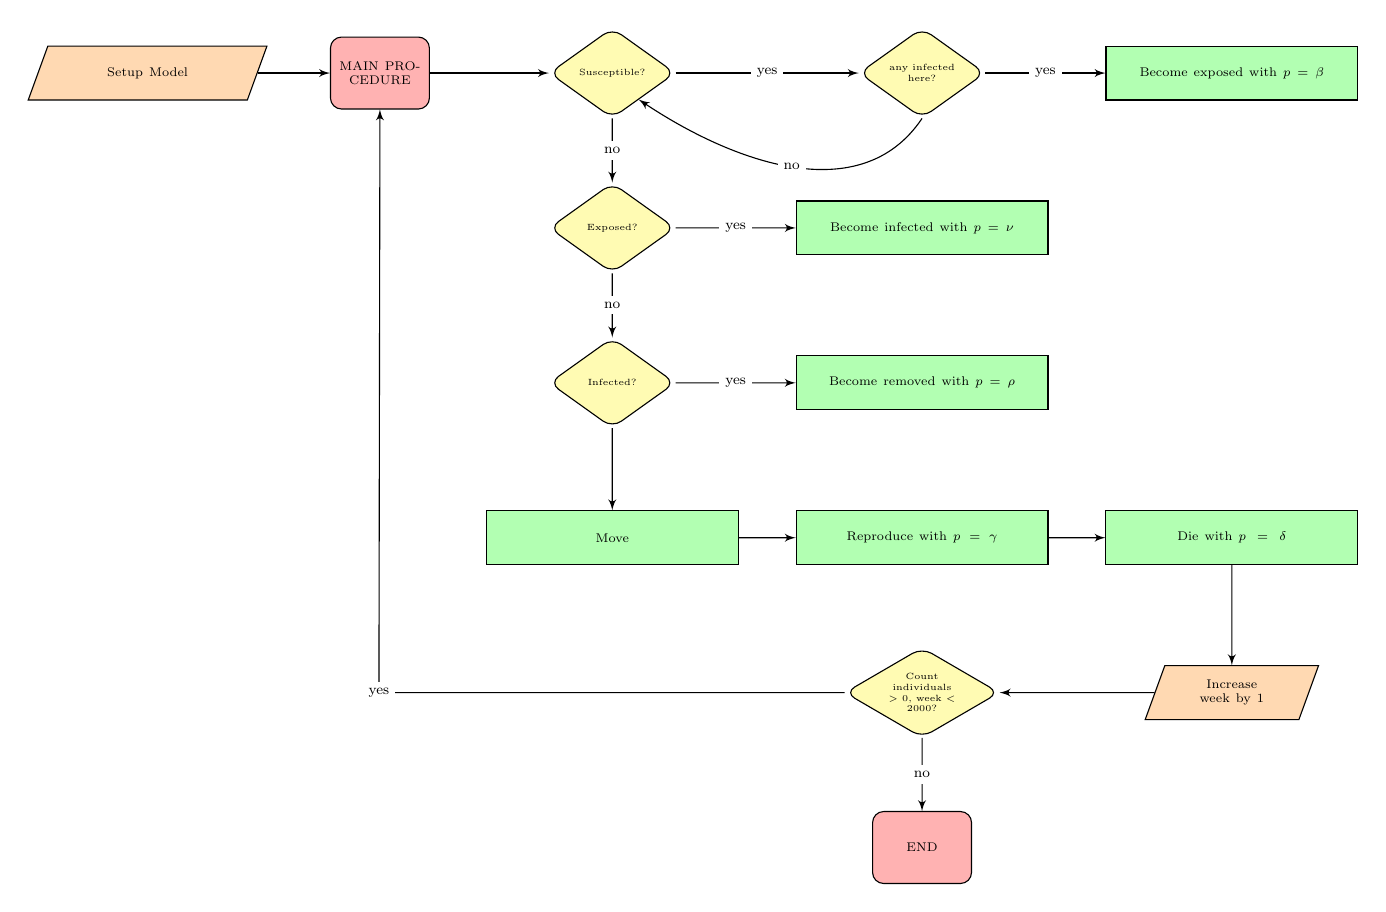
\begin{tikzpicture}[every node/.style={rectangle,fill=white,node distance=16ex, scale=0.65}, scale=0.90]
	% First row
	\node [io, fill=orange!30] (Setup) {Setup Model};
	\node [cloud, fill=red!30, right of=Setup, node distance = 30ex] (Main) {MAIN PROCEDURE};
	\node [decision, fill=yellow!30, right of = Main, node distance = 30ex] (Susceptible) {Susceptible?};
	\node[decision, fill=yellow!30, right of = Susceptible, node distance = 40ex](infecteds-here){any infected here?};
	\node [block, fill=green!30, right of = infecteds-here, node distance = 40ex] (become-exposed){Become exposed with $p = \beta$};
	
	% Second row
	\node[decision, fill=yellow!30, below of = Susceptible, node distance = 20ex](Exposed) {Exposed?};
	\node[block, fill=green!30, right of = Exposed, node distance = 40ex](become-infected){Become infected with $p = \nu$};
	
	% Third row
	\node[decision, fill=yellow!30, below of = Exposed, node distance = 20ex](Infected){Infected?};
	\node[block, fill=green!30, right of = Infected, node distance = 40ex](become-removed){Become removed with $p = \rho$};
	
	% Fourth row
	\node[block, fill=green!30, below of = Infected, node distance = 20ex](Move){Move};
	\node[block, fill=green!30, right of = Move, node distance = 40ex](Reproduce){Reproduce with $p = \gamma$};
	\node[block, fill=green!30, right of = Reproduce, node distance = 40ex](Die){Die with $p = \delta$};
	
	% Fifth row
	\node[io, fill=orange!30, below of = Die, node distance = 20ex](Week){Increase week by 1};
	\node[decision, fill=yellow!30, left of = Week, node distance = 40ex](Stop){Count individuals > 0, week < 2000?};
	
	% Sixth row
	\node[cloud, fill=red!30, below of = Stop, node distance = 20ex](End){END};
	
	% Paths
	\path [line] (Setup) -- (Main);
	\path [line] (Main) -- (Susceptible);
	\path [line] (Susceptible) -- node{\footnotesize yes} (infecteds-here);
	\path [line] (infecteds-here) -- node{\footnotesize yes} (become-exposed);
	\path [line] (infecteds-here.south) to [bend left=5, out=60, in=150] node{\footnotesize no} (Susceptible.315);
	\path [line] (Susceptible) -- node{\footnotesize no} (Exposed);
	\path [line] (Exposed) -- node{\footnotesize yes} (become-infected);
	\path [line] (Exposed) -- node{\footnotesize no} (Infected);
	\path [line] (Infected) -- node{\footnotesize yes} (become-removed);
	\path [line] (Infected) -- (Move);
	\path [line] (Move) -- (Reproduce);
	\path [line] (Reproduce) -- (Die);
	\path [line] (Die) -- (Week);
	\path [line] (Week) -- (Stop);
	\path [line] (Stop) -- node{\footnotesize no} (End);
	\path [line] (Stop.west) -- ++(-6.57,0) node{\footnotesize yes} -- (Main.south);
	\end{tikzpicture}
\end{figure}

\pagebreak

% Fairly complex
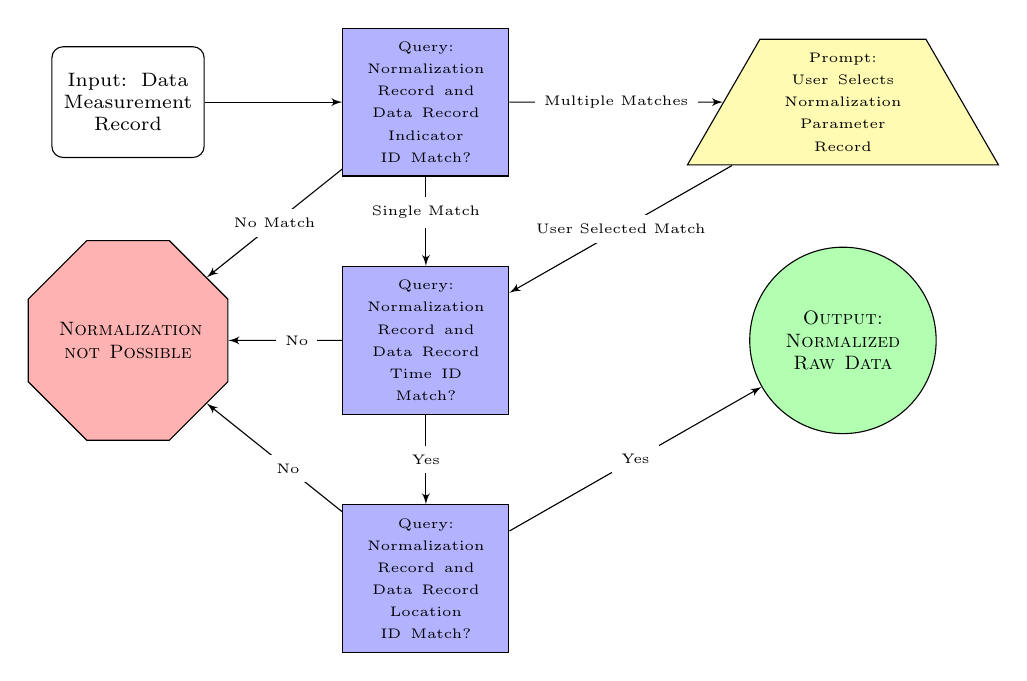
\begin{tikzpicture}[every node/.style={rectangle,fill=white,node distance=16ex}]
	%Place nodes
	\node [cloud, fill=white!30] (Input) {Input: Data Measurement Record};
	\node [query, fill=blue!30, right of=Input, node distance=25ex] (NormID?) {\tiny Query: Normalization Record and Data Record Indicator ID Match?};
	\node [prompt, fill=yellow!30, right of=NormID?, node distance=35ex] (Prompt) {\tiny Prompt: User Selects Normalization Parameter Record};
	\node [query, fill=blue!30, below of=NormID?, node distance=20ex] (TimeID?) {\tiny Query: Normalization Record and Data Record Time ID Match?};
	\node [query, fill=blue!30, below of=TimeID?, node distance=20ex] (LocationID?) {\tiny Query: Normalization Record and Data Record Location ID Match?};
	\node [go, fill=green!30, right of=TimeID?, node distance=35ex] (Normalize) {\textsc{Output: Normalized Raw Data}};
	\node [stop, fill=red!30, left of=TimeID?, node distance=25ex] (NotNormalize) {\textsc{Normalization not Possible}};
	
	\path [line] (Input) -- (NormID?);
	\path [line] (NormID?) -- node[pos=0.5] {\tiny Multiple Matches} (Prompt);
	\path [line] (NormID?) -- node[pos=0.4] {\tiny Single Match} (TimeID?);
	%\path [line] (NormID?.south) -- node[bend right=15] {\tiny No Match} (NotNormalize.30);
	\path [line] (NormID?) -- node[pos=0.5] {\tiny No Match} (NotNormalize);
	\path [line] (Prompt) -- node[pos=0.5] {\tiny User Selected Match} (TimeID?);

	%\path [line] (Prompt.south) to[bend left=15] (TimeID?.30);
	\path [line] (TimeID?) -- node[pos=0.5] {\tiny Yes} (LocationID?);
	\path [line] (TimeID?) -- node[pos=0.4] {\tiny No} (NotNormalize);
	\path [line] (LocationID?) -- node[pos=0.5] {\tiny Yes} (Normalize);
	\path [line] (LocationID?) -- node[pos=0.4] {\tiny No} (NotNormalize);
	
\end{tikzpicture}

\pagebreak

% The most complex one ever
\begin{landscape}
\begin{center}
  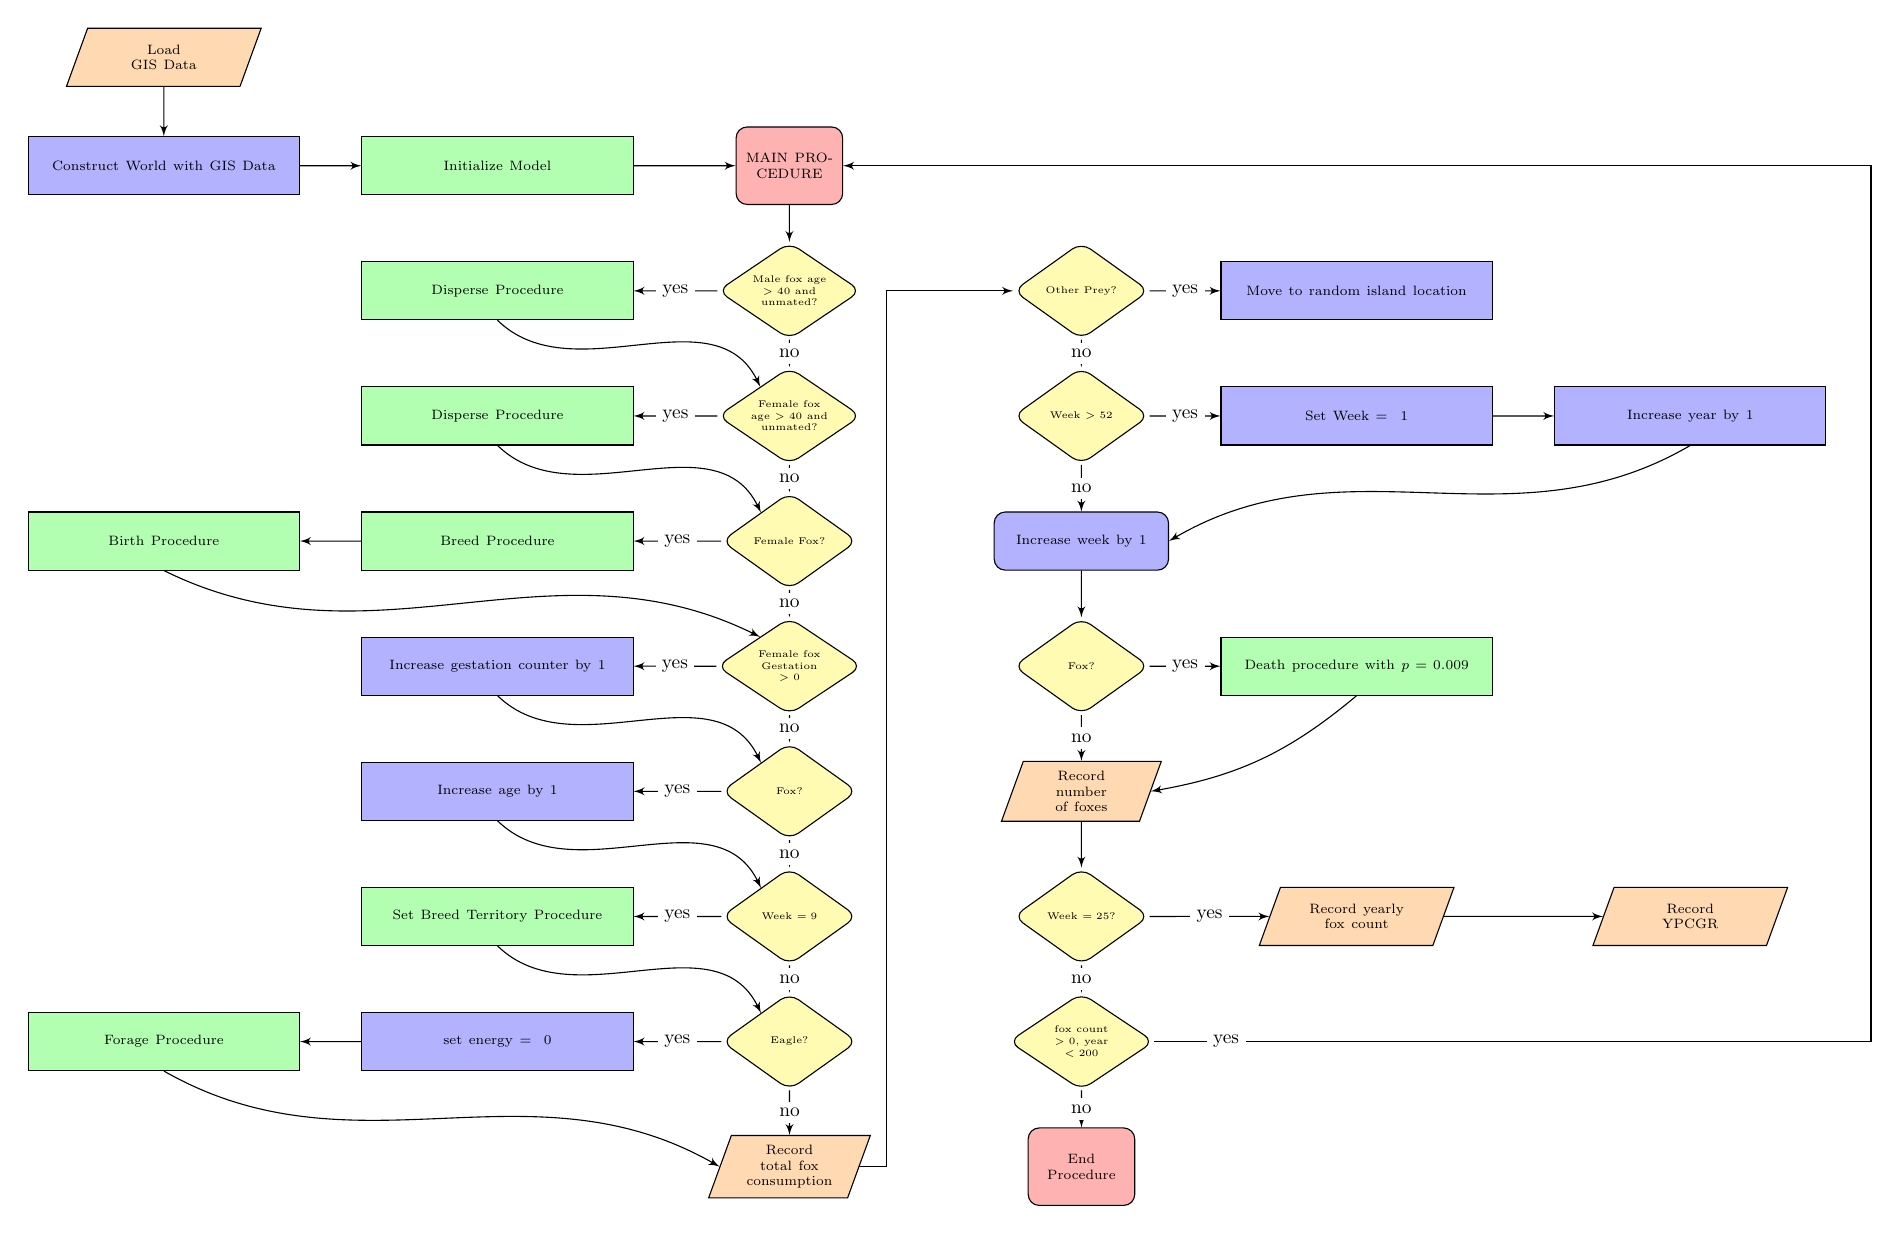
\begin{tikzpicture}[every node/.style={rectangle,fill=white,node distance=16ex, scale=0.70}, scale=0.70]
  %first column
   %node definitions
   %top row
   \node [io, fill=orange!30] (LoadGIS) {Load GIS Data};
   \node [block, fill=blue!30, below of=LoadGIS, node distance=13ex] (Construct) {Construct World with GIS Data};
   \node [block, fill=green!30, right of=Construct, node distance=40ex] (Initialize){Initialize Model};
   \node [cloud, fill=red!30, right of=Initialize, node distance=35ex] (Main) {MAIN PROCEDURE};
   %second row
   \node [block, fill=green!30, below of=Initialize, node distance=15ex] (DisperseM) {Disperse Procedure};
   \node [decision, fill=yellow!30, below of=Main, node distance=15ex] (Age?Mate?M) {Male fox age $>40$ and unmated?};
   %third row
   \node [block, fill=green!30, below of=DisperseM, node distance=15ex] (DisperseF) {Disperse Procedure};
   \node [decision, fill=yellow!30, below of=Age?Mate?M, node distance=15ex] (Age?Mate?F){Female fox age $>40$ and unmated?};
   %fourth row
   \node [block, fill=green!30, below of=DisperseF, node distance=15ex] (Breed) {Breed Procedure};
   \node [block, fill=green!30, left of=Breed, node distance=40ex] (Birth) {Birth Procedure};
   \node [decision, fill=yellow!30, below of=Age?Mate?F, node distance=15ex] (FemaleFox) {Female Fox?};
   %fifth row
   \node [block, fill=blue!30, below of=Breed, node distance=15ex] (IncGestation) {Increase gestation counter by $1$};
   \node [decision, fill=yellow!30, below of=FemaleFox, node distance=15ex] (FGest) {Female fox Gestation $>0$};
   %sixth row
   \node [block, fill=blue!30, below of=IncGestation, node distance=15ex] (IncAge) {Increase age by 1};
   \node [decision, fill=yellow!30, below of=FGest, node distance=15ex] (Fox?) {Fox?};
   %seventh row
   \node [block, fill=green!30, below of=IncAge, node distance=15ex] (BreedTerr) {Set Breed Territory Procedure};
   \node [decision, fill=yellow!30, below of=Fox?, node distance=15ex] (BWeek?) {Week $= 9$};
   %eighth row
   \node [block, fill=blue!30, below of=BreedTerr, node distance=15ex] (SetE) {set energy $= 0$};
   \node [block, fill=green!30, left of=SetE, node distance=40ex] (Forage) {Forage Procedure};
   \node [decision, fill=yellow!30, below of=BWeek?, node distance=15ex] (Eagle?) {Eagle?};
   %ninth row
   \node [io, fill=orange!30, below of=Eagle?, node distance=15ex] (FoxCon) {Record total fox consumption};
   
  %column two
   %first row
   \node [decision, fill=yellow!30, right of=Age?Mate?M, node distance=35ex] (OtherPrey) {Other Prey?};
   \node [block, fill=blue!30, right of=OtherPrey, node distance=33ex] (RandomMove) {Move to random island location};
   %second row
   \node [decision, fill=yellow!30, below of=OtherPrey, node distance=15ex] (OneYear?) {Week $>52$};
   \node [block, fill=blue!30, below of=RandomMove, node distance=15ex] (SetWeek) {Set Week $=1$};
   \node [block, fill=blue!30, right of=SetWeek, node distance=40ex] (IncYear) {Increase year by $1$};
   %third row
   \node [subcloud, fill=blue!30, below of=OneYear?, node distance=15ex] (IncWeek) {Increase week by $1$};
   %fourth row
   \node [decision, fill=yellow!30, below of=IncWeek, node distance=15ex] (Fox2) {Fox?};
   \node [block, fill=green!30, below of=SetWeek, node distance=30ex] (Death) {Death procedure with $p = 0.009$};
   %sixth row
   \node [io, fill=orange!30, below of=Fox2, node distance=15ex] (NumFoxes) {Record number of foxes};
   %seventh row
   \node [decision, fill=yellow!30, below of=NumFoxes, node distance=15ex] (Wk25) {Week $= 25$?};
   \node [io, fill=orange!30, below of=Death, node distance=30ex] (FoxCount) {Record yearly fox count};
   \node [io, fill=orange!30, below of=IncYear, node distance=60ex] (YPCGR) {Record YPCGR};
   \node [decision, fill=yellow!30, below of=Wk25, node distance=15ex] (StopCon) {fox count $> 0$, year $< 200$};
   \node[cloud, fill=red!30, below of=StopCon, node distance=15ex] (End) {End Procedure};
   
   %paths
   \path [line] (LoadGIS) -- (Construct);
   \path [line] (Construct) -- (Initialize);
   \path [line] (Initialize) -- (Main);
   \path [line] (Main) -- (Age?Mate?M);
   \path [line] (DisperseM.south) to [bend right=15, out=330, in=130] (Age?Mate?F.135);
   \path [line] (Age?Mate?M) -- node {yes} (DisperseM);
   \path [line] (Age?Mate?M) -- node {no} (Age?Mate?F);
   \path [line] (DisperseF.south) to [bend right=15, out=330, in=130] (FemaleFox.135);
   \path [line] (Age?Mate?F) -- node {yes} (DisperseF);
   \path [line] (Age?Mate?F) -- node {no} (FemaleFox);
   \path [line] (FemaleFox) -- node {yes} (Breed);
   \path [line] (FemaleFox) -- node {no} (FGest);
   \path [line] (Breed) -- (Birth);
   \path [line] (Birth.south) to [bend right=5, out=340, in=160] (FGest.135);
   \path [line] (FGest) -- node {yes} (IncGestation);
   \path [line] (FGest) -- node {no} (Fox?);
   \path [line] (IncGestation.south) to [bend right=15, out=330, in=130] (Fox?.135);
   \path [line] (Fox?) -- node {yes} (IncAge);
   \path [line] (Fox?) -- node {no} (BWeek?);
   \path [line] (IncAge.south) to [bend right=15, out=330, in=130] (BWeek?.135);
   \path [line] (BWeek?) -- node {yes} (BreedTerr);
   \path [line] (BWeek?) -- node {no} (Eagle?);
   \path [line] (BreedTerr.south) to [bend right=15, out=330, in=130] (Eagle?.135);
   \path [line] (Eagle?) -- node {yes} (SetE);
   \path [line] (Eagle?) -- node {no} (FoxCon);
   \path [line] (SetE) -- (Forage);
   \path [line] (Forage.south) to [bend right=5, out=340, in=160] (FoxCon.west);
   \path [line] (FoxCon.east) -- ++(0.5,0) |- (OtherPrey.west);
   \path [line] (OtherPrey) -- node {yes} (RandomMove);
   \path [line] (OtherPrey) -- node {no} (OneYear?);
   \path [line] (OneYear?) -- node {yes} (SetWeek);
   \path [line] (OneYear?) -- node {no} (IncWeek);
   \path [line] (SetWeek) -- (IncYear);
   \path [line] (IncYear.south) to [bend left=5, out=20, in=200] (IncWeek.east);
   \path [line] (IncWeek) -- (Fox2);
   \path [line] (Fox2) -- node {yes} (Death);
   \path [line] (Fox2) -- node {no} (NumFoxes);
   \path [line] (Death.south) to [bend left=15] (NumFoxes.east);
   \path [line] (NumFoxes) -- (Wk25);
   \path [line] (Wk25) -- node {yes} (FoxCount);
   \path [line] (Wk25) -- node {no} (StopCon);
   \path [line] (FoxCount) -- (YPCGR);
   \path [line] (StopCon) -- node {no} (End);
   
   \path [line] (StopCon.east) -- ++(13,0) node[pos=0.1] {yes} |- (Main.east);
  \end{tikzpicture}
\end{center}
\end{landscape}

\end{document}